\chapter{Partículas idénticas}
Supongamos tres osciladores armónicos 1D. Son partículas
idénticas\footnote{Dos partículas son idénticas si sus propiedades
  (masa, carga, etc.) son idénticas; ningún experimento podría
  diferenciarlas. Una consecuencia importante es que si un sistema
  contiene partículas idénticas, no hay ningún cambio en su evolución
  o propiedades si se intercambian entre ellas. Notar que si un
  obserbable es simétrico respecto a permutaciones de las partículas
  cuentan como idénticas a efectos de la medición.} con tres funciones de
onda en tres coordenadas:
\begin{equation}
 f(x_1),g(x_2),h(x_3)
\end{equation}
 Se mueven en el espacio
producto tensorial de sus subespacios,
\begin{equation}
  \mathcal{E} = \mathcal{E}_1 \otimes \mathcal{E}_2 \otimes \mathcal{E}_3 
\end{equation}
Puedo hallar una base de $\mathcal{E}$ del estilo $\{\varphi_i(x_1),
\varphi_j(x_2), \varphi_k(x_3)\}$, con un CSCO como
$ \Ham _1, \Ham _2,  \Ham _3$ al no haber degeneración
en el caso 1D. El problema es que al medir una energía no sé cual de
las tres he medido. Supongamos que mido tres energías
$E_5,E_7,E_{10}$, El sistema puede ser el
$\varphi_5(x_1)\varphi_7(x_2)\varphi_{10}(x_3)$, el
$\varphi_5(x_2)\varphi_7(x_3)\varphi_{10}(x_1)$ o cualquier otro. Hay $3!$ sistemas
distintos que darían esa medición, al no estar ``etiquetadas'' las
partículas; a esto lo llamamos \emph{degeneración de intercambio}.

Por lo visto el CSCO utilizado no es \emph{completo}, problema que
solucionamos con el \emph{postulado de simetrización}:

\begin{thm}[Postulado de simetrización]
  La función de ondas de un sistema de partículas idénticas es 
  simétrica o\footnotemark antisimétrica bajo una transposición $i
  \leftrightarrow j$.
\end{thm}

\footnotetext{Para el lector adverso al castellano y
    aficcionado a la lógica formal, $\Psi \in \Psi_\text{sim} \oplus
    \Psi_\text{anti}$:
    \begin{center}
      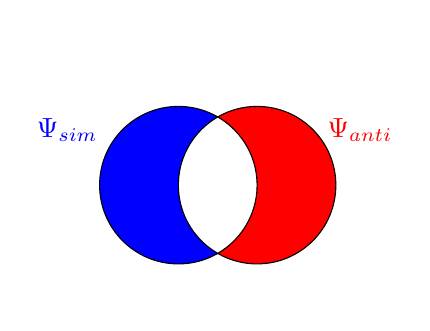
\begin{tikzpicture}[fill=red][xscale=0.6]
        % left hand
        \scope \clip (-1.5,-1.5) rectangle (2,2) (1,0) circle (1); \fill[blue]
        (0,0) circle (1);
        \endscope
        % right hand
        \scope \clip (-1.5,-1.5) rectangle (2,2) (0,0) circle (1); \fill[red]
        (1,0) circle (1);
        \endscope
        % outline
        \draw (0,0) circle (1) (0,1) (1,0) circle (1) (1,1);
        \node [text=blue,left] at (-0.9,0.7) {$\Psi_\text{sim}$}; 
        \node [text=red,right] at (+1.77,0.7) {$\Psi_\text{anti}$};
      \end{tikzpicture}
    \end{center}
donde $\oplus$ es la disyunción exclusiva.
}

Como solo hay una función de ondas simétrica (la suma de las
transposiciones) y otra antisimétrica (la suma de las transposiciones,
con el signo cambiado en las permutaciones impares) el estado del
sistema queda fijado, solucionando el problema de la degeneración de
intercambio. A las partículas con función de ondas simétrica
se les llama \emph{bosones}, y a las que tienen función de ondas
antisimétrica \emph{fermiones}\footnote{Aplicando la relatividad
  restringida, vemos que los bosones tienen espín entero y los
  fermiones semientero}. Por ejemplo, si tengo dos partículas 1D con
funciones de onda $\varphi(r) = \cos(r)$ y $\psi(r)=r^2$ la función de
ondas del sistema será $\Psi=\varphi(x)\psi(y)+\varphi(y)\psi(x)$ si son bosones
y $\Psi=\varphi(x)\psi(y)-\varphi(y)\psi(x)$ si son fermiones (puede verse el
aspecto de $\Psi(x,y)$ en la figura \ref{fig:simetry}).

\begin{figure}
  \centering
  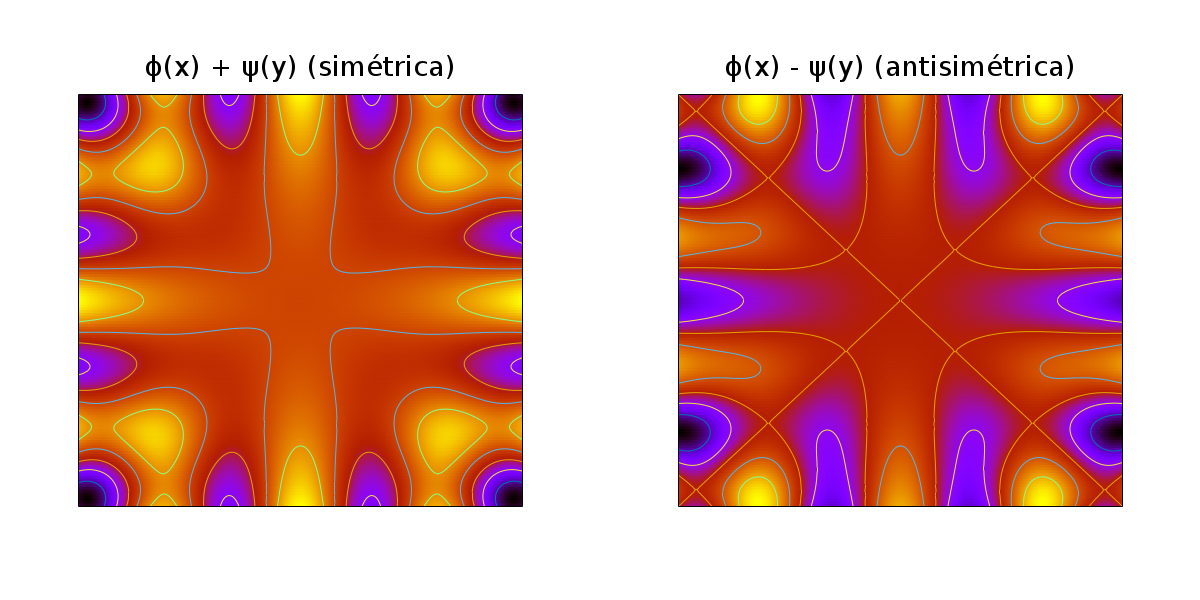
\includegraphics[width=\textwidth]{figures/simetry.png}
  \caption{Aspecto de una función de ondas simétrica y de una función de
    ondas antisimétrica}
  \label{fig:simetry}
  \forceversofloat
\end{figure}

Al ser el hamiltoniano simétrico\footnote{Al ser las partículas
  idénticas, las permutaciones de índices no deben tener un efecto
  real en las mediciones.} una función de ondas conserva su
simetría, como puede verse analizando la ecuación de Schrödinger ($i
\hbar \pdv{t} \psi =  \Ham \psi$).

\section{Partículas no elementales}
A veces es complicado definir
``partícula'', al no existir certeza absoluta sobre la ausencia de
estructura interna. Puede evitarse ese problema suponiendo al objeto
una partícula elemental y utilizando como espín el momento angular
total respecto al centro de masas, $J^*$; el hidrógeno, por ejemplo,
se comporta como una partícula elemental de espín
$s=J^*=\nicefrac{1}{2}\otimes\nicefrac{1}{2}\otimes l$. Al ser $l$
entero, el espín queda entero y se comporta como un bosón. De esta
forma, obtenemos los mismos resultados al permutar dos átomos de hidrógeno 
consideremos o no la estructura interna:
\begin{align}
  \psi &=
  \psi(\underset{p}{1},\underset{e^-}{2},\underset{p}{3},\underset{e^-}{4})
  \ \stackrel{1 \leftrightarrow 3}{\rightarrow} \ -\psi(3,2,1,4)  \
  \stackrel{2 \leftrightarrow 4}{\rightarrow} +\psi(3,4,1,2) \\
  \psi &=
  \psi(\underset{\text{H}_1}{1},\underset{\text{H}_2}{2})
  \ \stackrel{1 \leftrightarrow 2}{\rightarrow} \ +\psi(2,1)
\end{align}

%Redactar como una persona
Como ejemplos en la naturaleza tenemos el deuterio, el \textsuperscript{3}He
(ambos fermiones) y el \textsuperscript{4}He (un
bosón).\jokemargin{El \textsuperscript{3}He ha sido declarado recurso estratégico,
  de forma que EEUU ya lo ha acaparado. El Ministerio de Energía lo
  tiene todo y solo lo suelta bajo juramento y... bueno, ya sabéis
  cómo funciona el imperio\index{imperio}, para qué os voy a aburrir. Lo hizo Roma,
  lo hicimos nosotros, lo hizo Inglaterra y ahora lo hace EEUU.}
\section{Determinante de Slater}\index{Slater, determinante}
Sea un hamiltoniano $ \Ham (1,2,3) = h(1) +
h(2) + h(3)$. Sean $E_u,E_v,E_w$ los autovalores de $ \Ham $
con autoestados correspondientes $u,v,w$. Hay $3!$ autoestados
$u(i)v(j)w(k)$; si las partículas son bosones no hay más que sumarlos,
si son fermiones podemos utilizar el determinante de Slater para
obtener rápidamente la función de ondas antisimétrica:
\begin{equation}
  \Psi_\text{ant.} \propto
  \begin{vmatrix}
    u(1) & u(2) & u(3) \\
    v(1) & v(2) & v(3) \\
    w(1) & w(2) & w(3) 
  \end{vmatrix} = u(1)v(2)w(3) - \cdots
\end{equation}
Notar que hay que determinar la norma de la función resultante, que no
es más que $\sqrt{3!}$ al escogerse\footnote{No siempre tiene por qué ser así} autoestados
ortogonales. Si bien el
método es generalizable sin más que utilizar un determinante mayor a
sistemas de $N$ partículas, solo es válido cuando el hamiltoniano es
separable (las partículas son independientes):
\begin{equation}
  \Psi_\text{ant.} = \frac{1}{\sqrt{N!}}
  \begin{vmatrix}
    \varphi_1(1) & \cdots & \varphi_1(N) \\
    \vdots & \ddots & \vdots \\
    \varphi_N(1) & \cdots & \varphi_N(N) \\
  \end{vmatrix} 
\end{equation}
De aquí se deduce el \emph{principio de exclusión de Pauli}. Si dos
columnas son iguales (dos partículas están en el mismo estado) el
determinante se anula y la probabilidad de que el sistema esté en ese
estado cuántico es nula.
\section{Degeneración de intercambio}
Consideremos dos partículas idénticas no independientes, con
hamiltoniano $ \Ham (1,2) =  \Ham (2,1) \neq h(1) + h(2) $
simétrico. Obtenemos la siguiente ecuación de autovalores:
\begin{equation}
     \Ham (1,2) \varphi(1,2) = E \varphi(1,2)
\end{equation}
Puedo permutar los índices sin cambiar la energía:
\begin{equation}
     \Ham (2,1) \varphi(2,1) = E \varphi(2,1)
\end{equation}
Pero como el hamiltoniano es simétrico,
\begin{equation}
     \Ham (1,2) \varphi(2,1) = E \varphi(2,1)
\end{equation}
vemos que $ \Ham $ tiene por tanto dos autoestados con la misma
energía, $\varphi(1,2)$ y $\varphi(2,1)$. A esta degeneración se le denota
\emph{degeneración de intercambio} para diferenciarla de otras
degeneraciones como la que aparece de manera natural en un oscilador
armónico 2D.

%%% Local Variables:
%%% mode: latex
%%% TeX-master: "../resumen"
%%% End:
